% !TeX root=../main.tex

\chapter{پاسخ سوالات سری اول}

\href{https://drive.google.com/drive/folders/1BMXUcHZQBMV6n8P9XX5LD0nV40Ff3FDP?usp=drive_link}{Google Drive Folder}

% دستور زیر باعث عدم‌نمایش شماره صفحه در اولین صفحهٔ این فصل می‌شود.
%\thispagestyle{empty}
\section{ پاسخ سوال 1}
\subsection{قسمت اول، بخش الف}
برای محاسبه ابعاد ماتریس ها پس از ضرب دو ماتریس در یک دیگر، در صورتی که ابعاد ماتریس اول X برابر با $m * n$ و ابعاد ماتریس دوم Y برابر $u * v$ باشد، می توانیم از رابطه ی زیر استفاده می کنیم. 
\[
X_{m \times n} \cdot Y_{u \times v} = Z_{m \times v}
\]
برای ماتریس های داده شده داریم:
\[
size(A) = 2*3 , size(B) = 4*2
\]
در نتیجه، سایز ماتریس های داده شده برابر خواهد بود با:
\[
size(B \times A) = 4*3 
\]
\[
size(B^{T}) = 2*4 
\]
\[
size(B^{T} \times A) = Null 
\]
\[
size(A^{T} \times B) = Null 
\]
ماتریس هایی که قابل ضرب شدن نیستند، به دلیل تناقض در ابعاد ماتریس ها و عدم همخوانی تعداد ستون های ماتریس اول با تعداد سطر های ماتریس دوم می باشد.

\subsection{قسمت اول، بخش ب}
ماتریس های مطرح شده در بخش قبل به صورت زیر خواهند بود.
\[
BA =
\begin{bmatrix}
	b_{11} & b_{12} \\
	b_{21} & b_{22} \\
	b_{31} & b_{32} \\
	b_{41} & b_{42}
\end{bmatrix}
\begin{bmatrix}
	a_{11} & a_{12} & a_{13} \\
	a_{21} & a_{22} & a_{23}
\end{bmatrix}
=
\begin{bmatrix}
	b_{11} a_{11} + b_{12} a_{21} & b_{11} a_{12} + b_{12} a_{22} & b_{11} a_{13} + b_{12} a_{23} \\
	b_{21} a_{11} + b_{22} a_{21} & b_{21} a_{12} + b_{22} a_{22} & b_{21} a_{13} + b_{22} a_{23} \\
	b_{31} a_{11} + b_{32} a_{21} & b_{31} a_{12} + b_{32} a_{22} & b_{31} a_{13} + b_{32} a_{23} \\
	b_{41} a_{11} + b_{42} a_{21} & b_{41} a_{12} + b_{42} a_{22} & b_{41} a_{13} + b_{42} a_{23}
\end{bmatrix}
\]

\[
B^T =
\begin{bmatrix}
	b_{11} & b_{21} & b_{31} & b_{41} \\
	b_{12} & b_{22} & b_{32} & b_{42}
\end{bmatrix}
\]


\subsection{قسمت دوم، بخش اول}
با در نظر داشتن ابعاد ماتریس x برابر با $1*2$ و ابعاد ماتریس $\theta$ برابر با $2*1$، ابعاد ماتریس $x*\theta$ برابر با $1*1$ خواهد بود.
با افزایش تعداد نمونه ها در سطر های جدیدی برای ماتریس 
\textbf{X}،
ابعاد ماتریس 
$\textbf{X} \times \theta$
برابر 
$n*1$
خواهد بود.
\subsection{قسمت دوم، بخش دوم}
\[
X\theta - \vec{y} =
\begin{bmatrix}
	x^{(1)T}\theta \\
	\vdots \\
	x^{(n)T}\theta
\end{bmatrix}
-
\begin{bmatrix}
	y^{(1)} \\
	\vdots \\
	y^{(n)}
\end{bmatrix}
=
\begin{bmatrix}
	h_\theta(x^{(1)}) - y^{(1)} \\
	\vdots \\
	h_\theta(x^{(n)}) - y^{(n)}
\end{bmatrix}.
\]

آنگاه با در نظر داشتن آنکه \( z \), خواهیم داشت \( z^T z = \sum_i z_i^2 \):

\[
\frac{1}{2}(X\theta - \vec{y})^T(X\theta - \vec{y}) = \frac{1}{2}\sum_{i=1}^{n}(h_\theta(x^{(i)}) - y^{(i)})^2 = J(\theta)
\]

سپس، برای کاهش مقدار \( J \) مشتق آن را نسبت به \( \theta \) به دست می آوریم.

\[
\nabla_\theta J(\theta) = \nabla_\theta \frac{1}{2}(X\theta - \vec{y})^T(X\theta - \vec{y})
\]

\[
= \frac{1}{2}\nabla_\theta \left( (X\theta)^T X\theta - (X\theta)^T\vec{y} - \vec{y}^T (X\theta) + \vec{y}^T\vec{y} \right)
\]

\[
= \frac{1}{2}\nabla_\theta \left( \theta^T (X^T X)\theta - \vec{y}^T (X\theta) - \vec{y}^T (X\theta) \right)
\]

\[
= \frac{1}{2}\nabla_\theta \left( \theta^T (X^T X)\theta - 2(X^T\vec{y})^T\theta \right)
\]

\[
= \frac{1}{2} \left( 2X^T X\theta - 2X^T\vec{y} \right)
\]

\[
= X^T X\theta - X^T\vec{y}
\]

\section{پاسخ سوال 2}
\subsection{پرده اول}
با در اختیار داشتن فرمول احتمال بیز به صورت زیر خواهیم داشت:
\[
P(+) = P(+ \cap \text{sick}) + P(+ \cap \text{$not sick$})
\]
در این رابطه، احتمال کل مثبت بودن نتیجه آزمایش در حالت مریض بودن یا نبودن محاسبه می شود. 
\[
P(+) = P(+ | \text{sick}) P(\text{sick}) + P(+ | \text{$not sick$}) P(\text{$not sick$})
\]
با جایگذاری مقادیر عددی خواهیم داشت:
\[
P(+) = \frac{99}{100} \cdot 10^{-4} + \frac{1}{100} \cdot \frac{9999}{10000} = 0.0010098
\]
حال با استفاده از فرمول بیز خواهیم داشت:
\[
P(\text{sick} | +) = \frac{P(+ | \text{sick}) P(\text{sick})}{P(+)}
\]
\[
P(\text{sick} | +) = \frac{0.000099}{0.0010098} \approx 0.0980392
\]

\subsection{پرده دوم}
در این پرده، به محاسبه ی احتمال بیمار بودن علی در صورتی که پاسخ هر دو تست مثبت باشند خواهیم پرداخت.

\[
P(\text{sick} | ++) = ?
\]
مجددا با استفاده از قانون احتمال کل خواهیم داشت:
\[
P(++) = P(++ | \text{sick}) P(\text{sick}) + P(++ | \text{$not sick$}) P(\text{$not sick$})
\]
که با جایگذاری مقادیر احتمال ها خواهیم داشت:
\[
P(++) = \frac{99}{100} \cdot \frac{9999}{10000} \cdot 10^{-4} + \frac{1}{100} \cdot \frac{1}{10000} \cdot \frac{9999}{10000}
\]
\[
= 0.00009899 + 0.00000000999
\]
\[
= 0.000099999 \approx 0.0001
\]
در پایان، با استفاده از رابطه ی بیز چنین به دست می آوریم:
\[
P(\text{sick} | ++) = \frac{P(++ | \text{sick}) P(\text{sick})}{P(++)}
\]
در اینجا خواهیم داشت:
\[
P(\text{sick} | ++) = \frac{P(++ | \text{sick}) P(\text{sick})}{P(++)}
\]
و با جایگذاری مقادیر به دست آمده در رابطه ی بالا خواهیم داشت:
\[
= \frac{0.989901 \times 10^{-4}}{0.0001}
\]
\[
= 0.9899
\]
\[
P(\text{sick} | ++) \approx 0.9899
\]
\subsection{پرده سوم}
\[
P(\text{sick} | ++-) = \frac{P(++- | \text{sick}) P(\text{sick})}{P(++-)}
\]
ابتدا به محاسبه ی  \( P(++-) \) می پردازیم:
\[
P(++-) = P(++- | \text{sick}) P(\text{sick}) + P(++- | \text{$not sick$}) P(\text{$not sick$})
\]
با جایگذاری مقادیر به دست می آوریم:
\[
= (0.99 \cdot 0.9999 \cdot 0.000001) \cdot 10^{-4} + (0.01 \cdot 0.0001 \cdot \frac{999999}{1000000}) \cdot \frac{9999}{10000}
\]
\[
= 0.000000989901 \cdot 0.0001 + 0.000000999 \cdot 0.9999
\]
\[
\approx 0.000000998
\]
\[
P(\text{sick} | ++-) = \frac{0.000000989901 \cdot 10^{-4}}{0.000000998}
\]
\[
\approx 9.918847 \cdot 10^{-5}
\]
\section{پاسخ سوال 3، قسمت اول}
\subsection{بخش الف، دریافت داده}
\subsubsection{1}
برای این قسمت، فایل 149 از مجموعه داده های قرار داده شده در سایت توسط نرم افزار های مدیریت دانلود، دانلود می شود. فرمت این فایل $.mat$ است.
برای استفاده از این فایل، ابتدا آن را در فضای ابری درایو ذخیره کرده و با ایجاد دسترسی برای آن فایل و استفاده از دستور gdown، آن را در محیط گوگل کولب وارد می کنیم. 
در ادامه، با استفاده از دستور loadmat از پکیج scipy.io، می توانیم دیتا را در یک متغیر ذخیره می کنیم. 
\begin{minted}{python}
!pip install --upgrade --no-cache-dir gdown

!gdown 1zKj4N5nFFKK1u9AhzlqJLvsw-xRC0kz_

from scipy.io import loadmat
file_path = '/content/149.mat'
mat_data = loadmat(file_path)
\end{minted}
\subsubsection{2}
پس از ذخیره سازی فایل، در متغیر بالا، می توانیم به جستجو درباره ویژگی های آن بپردازیم. با استفاده از دستور type مشاهده می کنیم که متغیر ذخیره شده از جنس dictionary است.
یک دیکشنری متشکل از بخش های زیر است:
\begin{enumerate}
	\item \textbf{Key} 
	کلید، مشخصه ای منحصر به فرد به ازای هر مقدار در دیکشنری است.
	\item \textbf{value}
	حاوی مقدار عددی مرتبط با یک key است و می تواند مقادیر تکراری داشته باشد.
	\item \textbf{item}
	به زوج key و value متناظر آن یک item گفته می شود و با علامت $:$ با یکدیگر مرتبط می شوند.
\end{enumerate}
\subsubsection{3}
در این بخش، با مشاهده ی کلید های موجود در دیکشنری سیستم خواهیم دید که این مجموعه داده توسط کلید های زیر تعریف شده اند.
\_\_header\_\_, \_\_version\_\_, \_\_globals\_\_, X149\_DE\_time, X149\_FE\_time, X149RPM
و از میان این مقادیر، دو سیگنال $X149\_DE\_time$ و $X149\_FE\_time$ حاوی سیگنال های اطلاعات هستند. در این بخش سیگنال $X149\_DE\_time$ انتخاب و در متغیری ذحیره می شود.
\subsection{بخش ب، نمایش سیگنال}
برای نمایش سیگنال انتخاب شده، لازم از کتابخانه ی Matplotlib استفاده شود. برای نمایش سیگنال، علاوه بر در اختیار داشتن خود سیگنال باید مقدار محور افقی که در این سوال برابر با زمان خواسته شده است نیز محاسبه شود. با در نظر داشتن فرکانس نمونه برداری برابر با 480000، مقادیر محور افقی با استفاده از دستور linspace در پکیج numpy ایجاد می شود. با تنظیم ابعاد نمودار مورد نظر با استفاده از دستور figure و تعیین ابعاد نمودار، می توانیم نمودار مورد نظر را نمایش دهیم.
\begin{minted}{python}
import numpy as np
import matplotlib.pyplot as plt

fs = 48000 #KHz
time = np.linspace(0, len(DE_time)/fs , len(DE_time))

plt.figure(figsize=(30,5))
plt.plot(time, DE_time)
plt.xlab
("Time(s)")
plt.ylabel("AMplitude")
plt.title("Signal of X149_DE_time")
plt.grid(True)
plt.show()
\end{minted}
با اجرای این کد، نمودار سیگنال به صورت زیر نمایش داده می شود.
% TODO: \usepackage{graphicx} required
\begin{figure}[H]
	\centering
	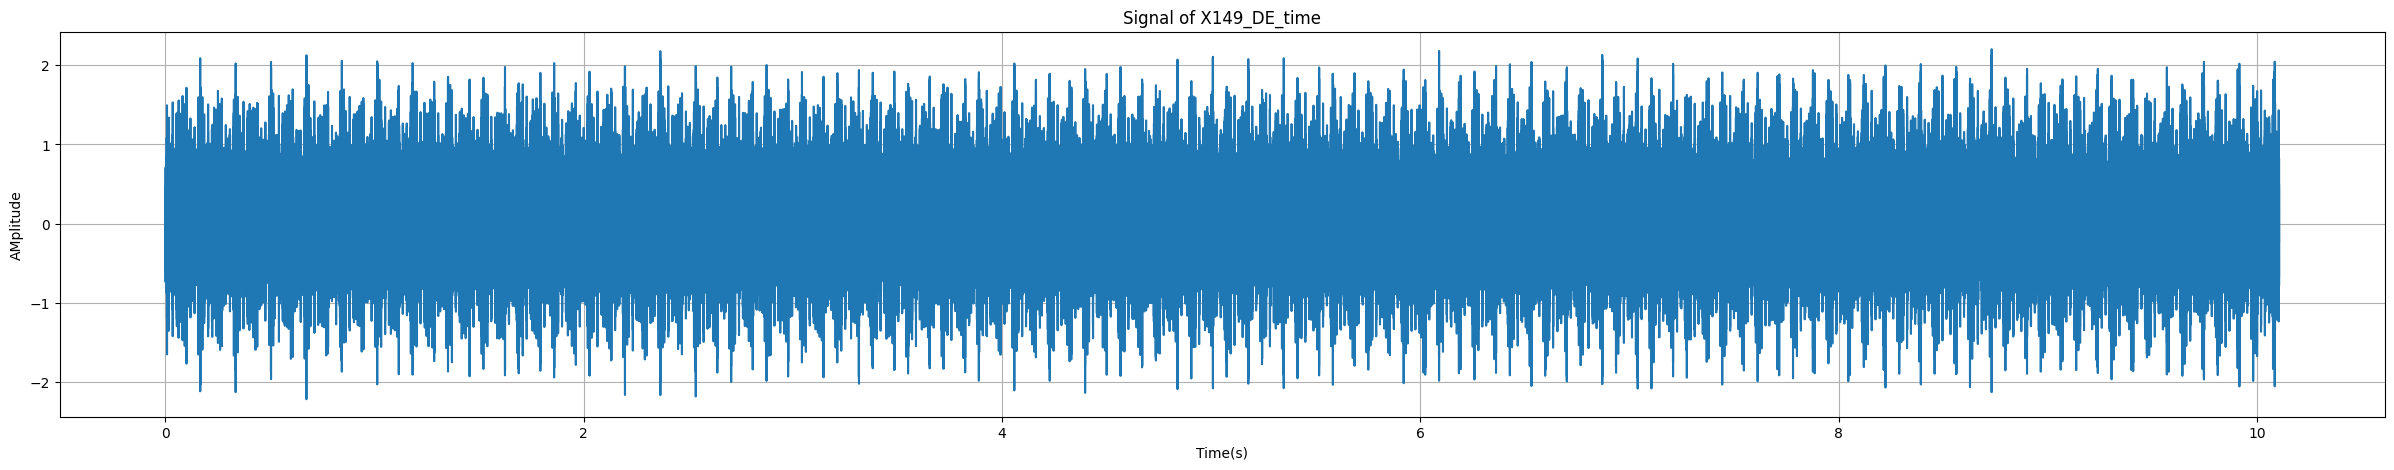
\includegraphics[width=1\linewidth]{../img/1}
	\caption{نمودار سیگنال $X149_DE_time$}
	\label{fig:1_}
\end{figure}

در بخش بعد، با محدود کردن ناحیه ی x در نمودار بین بازه ی 2 تا 2.01 ثانیه، سیگنال را مشاهده می کنیم.
\begin{minted}{python}
time = np.linspace(0, len(DE_time)/fs, len(DE_time))
plt.figure(figsize=(30, 5))
plt.plot(time, DE_time)
plt.xlabel("Time(s)")
plt.xlim(2, 2.01)
plt.ylabel("Amplitude") 
plt.title("Signal of X149_DE_time")
plt.grid(True)
plt.show()
\end{minted}
% TODO: \usepackage{graphicx} required
\begin{figure}[H]
	\centering
	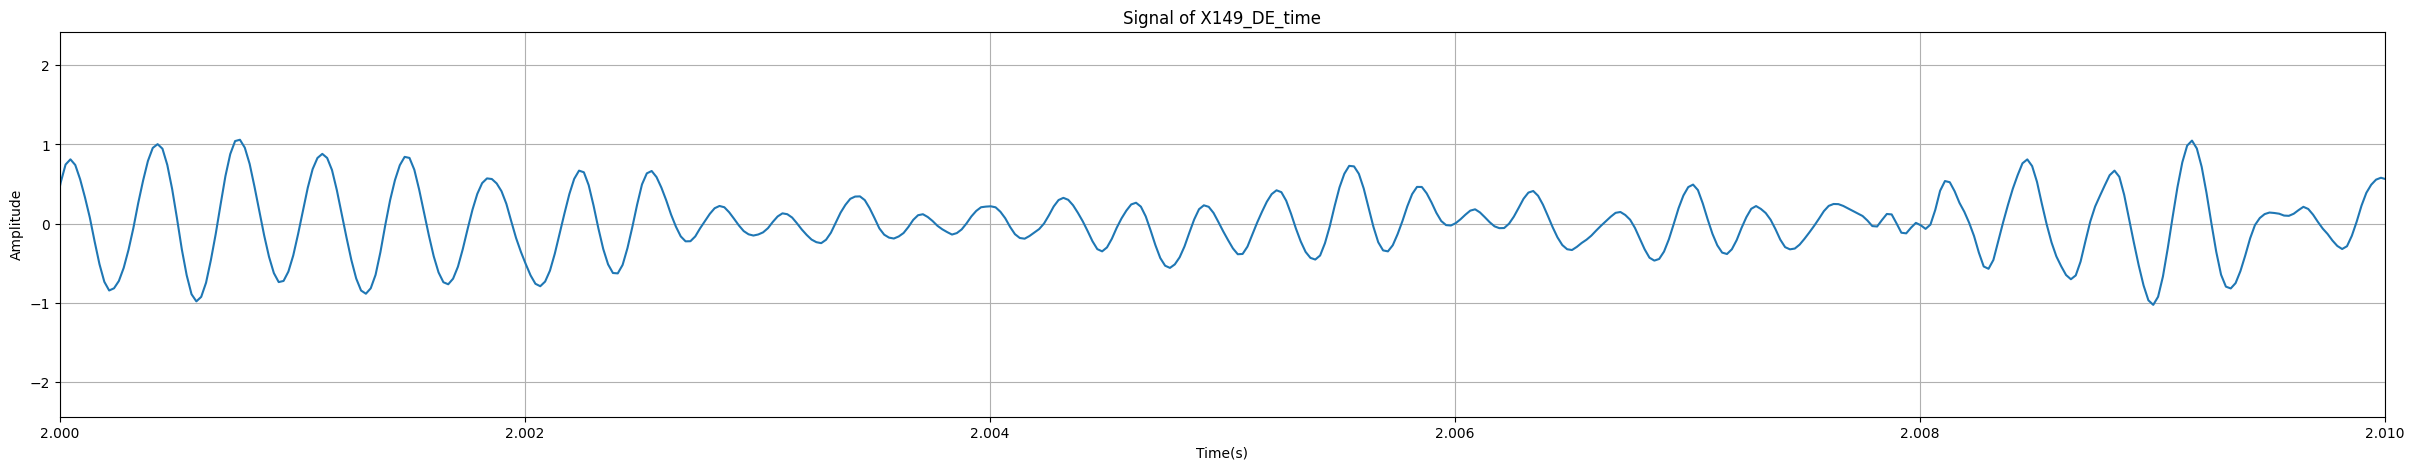
\includegraphics[width=1\linewidth]{../img/2}
	\caption{نمودار در بازه  ی2 تا $2.01$ ثانیه}
	\label{fig:2_}
\end{figure}

\subsection{بخش ج، تحلیل فرکانسی}
در این بخش، تابعی برای محاسبه ی تبدیل فوریه نوشته می شود. در نوشتن این تابع از روش fft در پکیج numpy استفاده شده است و پس از مشخص کردن فرکانس نمونه برداری داده ها، نمودار حوزه فرکانس سیستم رسم شده است.


% TODO: \usepackage{graphicx} required
\begin{figure}
	\centering
	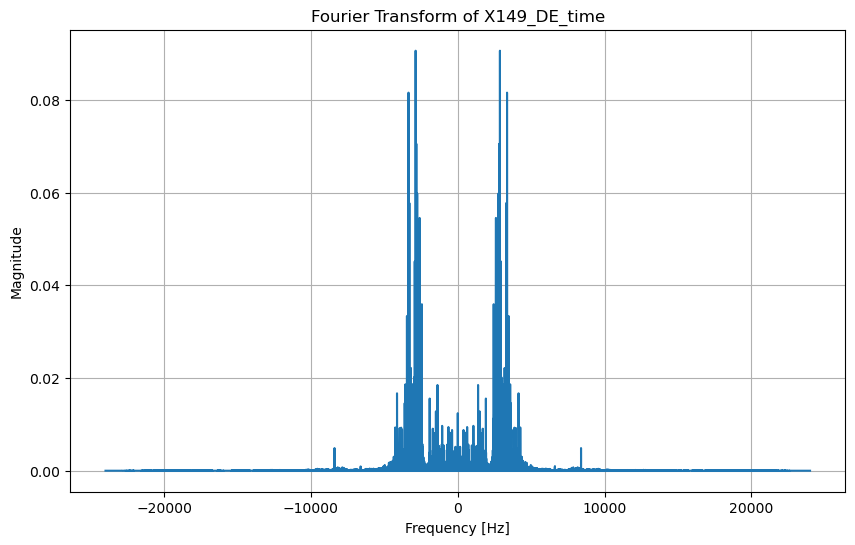
\includegraphics[width=1\linewidth]{../img/3}
	\caption{نمودار حوزه فرکانس سیگنال مورد بررسی}
	\label{fig:3_}
\end{figure}
همچنین، با اندازه گیری فرکانس با بیشترین دامنه، فرکانس غالب سیستم را برابر با
$3201 Hz$ به دست می آوریم.

\subsection{بخش د و ه، تقسیم بندی سیگنال}
برای تقسیم سیگنال به سطر هایی با 128 نمونه، از دستور reshape استفاده می کنیم. با این حال، باید توجه داشته باشیم که تعداد داده ها باید حتما بر 128 بخش پذیر باشند و بنابراین، پیش از اعمال دستور reshape، سیگنال را به تعدادی بخش پذیر بر 128 برش می دهیم. 
در نهایت، ماتریسی به صورت زیر به دست می آید.
\begin{minted}{python}
num_sections = len(DE_time) // 128
signal_trimmed = DE_time[:num_sections * 128]
sections = signal_trimmed.reshape(-1,128)
df = pd.DataFrame(sections)
df
\end{minted}
\begin{figure}
	\centering
	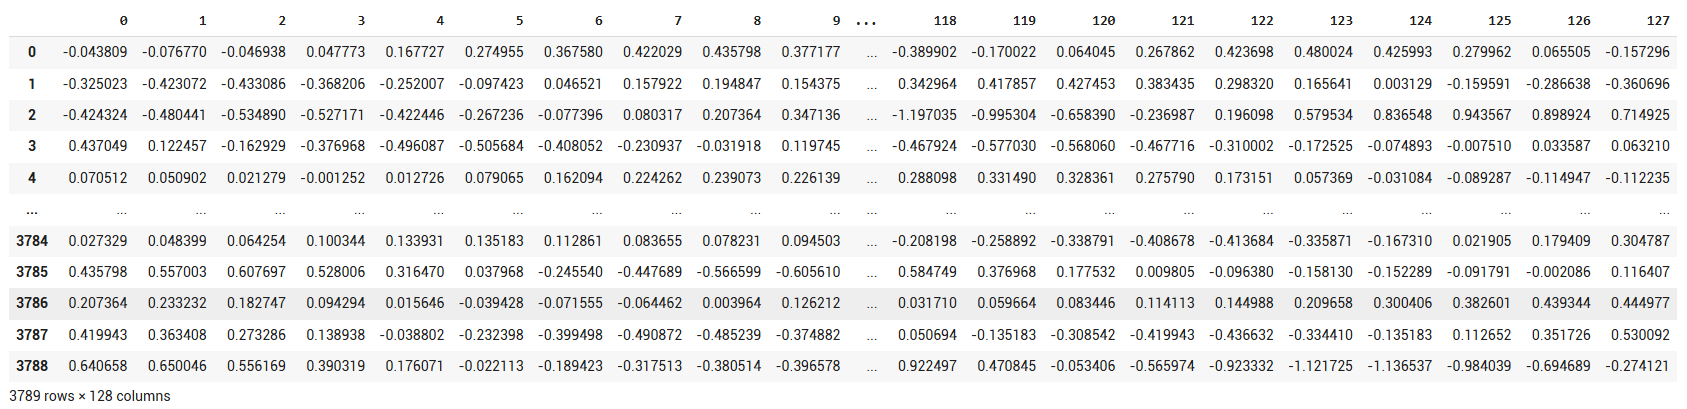
\includegraphics[width=1\linewidth]{../img/4}
	\caption{دیتافریم بخش های سیستم}
	\label{fig:4_}
\end{figure}

در نهایت، برای رسم نمودار بخش های انتخاب شده از سیگنال، با استفاده از کتابخانه ی matplotlib، آنها را در یک حلقه ی for به نمودار اضافه کرده و در نهایت نمودار را نمایش می دهیم. لازم به ذمر است که برای اضافه کردن legend به سیستم نیز، برای هر نمودار label متناسب تولید کرده و در نهایت، آن را در legend نمایش می دهیم.
\begin{minted}{python}
plt.figure(figsize=(10, 5))
for i in range(10):
var = df.iloc[13*i]
var = np.array(var).reshape(var.shape[0], -1)  
plt.plot(np.arange(len(var)), var.flatten(), label=f"Section {i+1}")  
plt.title("Sections")
plt.xlabel("Samples")
plt.ylabel("Value")
plt.legend(loc="center left", bbox_to_anchor=(1, 0.5)) 
plt.tight_layout()  
plt.show()
\end{minted}
نمودار به دست آمده آنگاه به صورت زیر خواهد بود.
\begin{figure}[H]
	\centering
	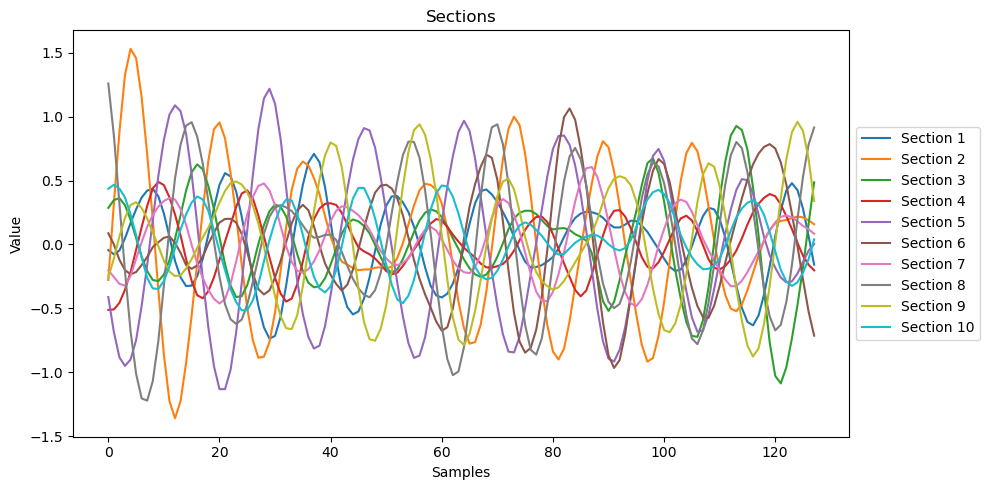
\includegraphics[width=1\linewidth]{../img/5}
	\caption{نمودار بخش های جدا شده از سیستم بر حسب زمان}
	\label{fig:5_}
\end{figure}

\subsection{بخش و، استخراج ویژگی}
در این قسمت، ویژگی های میانگین، انحراف معیار و RMS را با استفاده از روش های موجود در کتابخانه ی numpy محاسبه می کنیم. برای این کار، در یک class، تابع های مورد نیاز را تعریف کرده و سپس در پایان آن، در تابع main، هر سه را فراخوانی می کنیم. برای محاسبه ی میانگین و انحراف معیار از روش های آماده در کتابخانه ی numpy استفاده شده و RMS به صورت مجزا تعریف شده است.

\begin{minted}{python}
class Statistics:
def __init__(self, signal):
self.signal = np.array(signal)

def mymean(self):
return np.mean(self.signal)

def mystddev(self):
return np.std(self.signal)

def myRMS(self):
return np.sqrt(np.mean(np.square(self.signal)))

def main(signal):
stats = Statistics(signal)
print("Mean:", stats.mymean())
print("Standard Deviation:", stats.mystddev())
print("RMS:", stats.myRMS())
\end{minted}
	
آنگاه با فراخوانی این تابع و اعمال ورودی سیگنال به آن، می توانیم جدول ویژکی ها را محاسبه کنیم.

برای ایجاد ویژگی های خواسته شده برای تمام نمونه ها در دیتافریم، با فرض اینکه آن ستون ها وجود دارند، مقادیر را مطابق با روش های موجود در کلاس ساخته شده و به وسیله ی $lamda function$ می نویسیم.
\begin{minted}{python}
	df['Mean'] = df.apply(lambda row: Statistics(row.values).mymean(), axis = 1)
\end{minted}
	
\begin{minted}{python}
df['Standard Deviation'] = df.apply(lambda row: Statistics(row.values).mystddev(), axis = 1)
df['RMS'] = df.apply(lambda row: Statistics(row.values).myRMS(), axis = 1)
df
df.tocsv("dataset.csv", index=False)
\end{minted}
در پایان، دیتافریم به صورت زیر قابل مشاهده خواهد بود.
\begin{figure}[H]
	\centering
	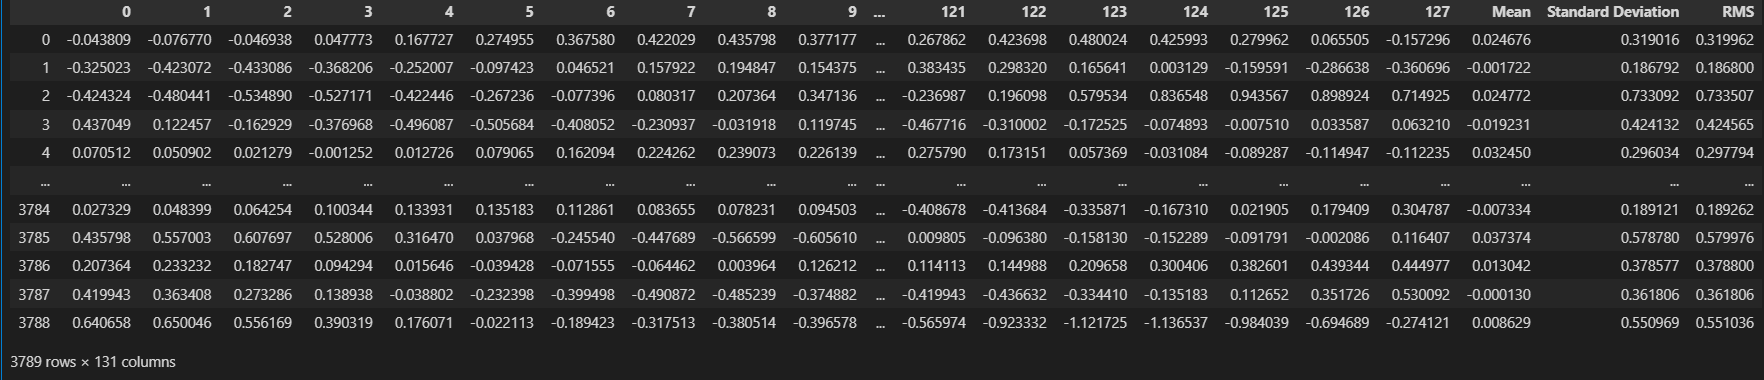
\includegraphics[width=1\linewidth]{../img/6}
	\caption{دیتافریم پس از استخراج ویژگی}
	\label{fig:6}
\end{figure}
در نهایت، دیتافریم را در یک فایل csv ذخیره می کنیم.
\section{پاسخ سوال سوم، قسمت دوم}
\subsection{بخش اول، بررسی اولیه}
دیتاست گل زنبق اولین بار توسط رونالد فیشر در کتابش معرفی شد و شامل داده های 150 نمونه گل زنبق است. ویژگی های اندازه گیری شده برای این گل ها به شرح زیر است:
\begin{enumerate}
	\item Sepal Length
	\item Sepal Width
	\item Petal Length
	\item Petal Width
\end{enumerate}
که مربوط به ابعاد اجزای گل ها می باشد. علاوه بر این، سه کلاس مختلف این گل ها به صورت زیر در این دیتاست نام گذاری شده اند:
\begin{enumerate}
	\item 0: Setosa
	\item 1: Versicolor
	\item 2: Virginica
\end{enumerate}

از ویژگی های بارز این دیتاست آن است که به ازای هر کلاس، دقیقا 50 نمونه داده وجود دارد که دیتاست را متعادل می سازد. علاوه بر این، داده ی خالی ندارد و همچنین کلاس Setosa به صورت خطی قابل جداسازی است.
برای استفاده از این دیتاست، می توانیم آن را از کتابخانه ی scikit-learn فراخوانی کنیم. در این دستور، از مجموعه داده های موجود در کتابخانه ی $scikit-learn$ دیتاست Iris را فراخوانده و سپس آن را در یک دیتافریم ذخیره می کنیم.
\begin{minted}{python}
	from sklearn import datasets
	import pandas as pd
	
	# Load dataset
	iris = datasets.load_iris()
	df = pd.DataFrame(iris.data, columns=iris.feature_names)
	df['species'] = iris.target
	
	print(df.head())
\end{minted}
% TODO: \usepackage{graphicx} required
\begin{figure}[H]
	\centering
	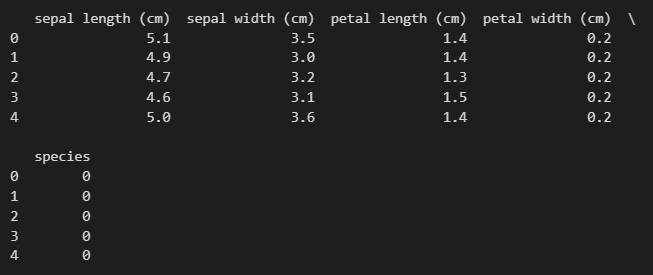
\includegraphics[width=0.7\linewidth]{../img/7}
	\caption{نمونه داده ی دیتاست زنبق}
	\label{fig:7}
\end{figure}

در ادامه برای تقسیم دیتاست به بخش آموزشی و تست، با استفاده از روش $Train_Test_split$ از کتابخانه ی sklearn در بخش $model_selection$ داده ها را به دو بخش تقسیم می کنیم. در اینجا ابتدا مقادیر فیچرها و کلاس های خروجی را به عنوان ورودی و خروجی سیستم تعریف کرده و سپس با استفاده از دستور ذکر شده، آنها را تقسیم می کنیم.
\begin{minted}{python}
	from sklearn.model_selection import train_test_split
	
	X = iris.data
	y = iris.target
	
	X_train, X_test, y_train, y_test =
	train_test_split(X,y, test_size=0.15, random_state=43) 
\end{minted}
در ادامه، نام ستون های متغیر های به دست آمده را باید مجدد نام گذاری کنیم و البته آنها را در دیتافریم هایی ذخیره کنیم.
\begin{minted}{python}
X_train = pd.DataFrame(X_train)
X_train.rename(columns={0:'Sepal Length',
 1:"Sepal Width",
 2:"Petal Length",
 3:"Petal Width"},inplace=True)

X_test = pd.DataFrame(X_test)
X_test.rename(columns={0:'Sepal Length',
 1:"Sepal Width",
 2:"Petal Length",
 3:"Petal Width"},inplace=True)

y_train = pd.DataFrame(y_train)
y_train.rename(columns={0:'Iris Type'},inplace=True)

y_test = pd.DataFrame(y_test)
y_test.rename(columns={0:'Iris Type'},inplace=True)

\end{minted}

در نهایت، دیتافریم های آموزش و تست را با به هم پیوستن داده های x و y آنها به وسیله دستور concat ترکیب می کنیم. 
\begin{minted}{python}
Train_df = pd.concat([X_train,y_train], axis=1)
Test_df = pd.concat([X_test,y_test], axis=1)
\end{minted}
برای مشخص کردن آنکه داده ها، مربوط به تست و یا آموزش هستند، ستونی به هر یک از دیتافریم ها با عنوان $is train$ اضافه شده که برای داده های train دارای مقدار 1 و برای داده های تست دارای مقدار 0 است.
در نهایت، با استفاده ی مجدد از دستور concat و به هم پیوستن این دو دیتافریم، دیتاست به صورت زیر به دست می آید.
\begin{minted}{python}
temporary_train = Train_df
temporary_train["is train"] = 1
temporary_test = Test_df
temporary_test["is train"] = 0

Dataset = pd.concat([temporary_train,temporary_test],ignore_index=True)
\end{minted}
\begin{figure}[H]
	\centering
	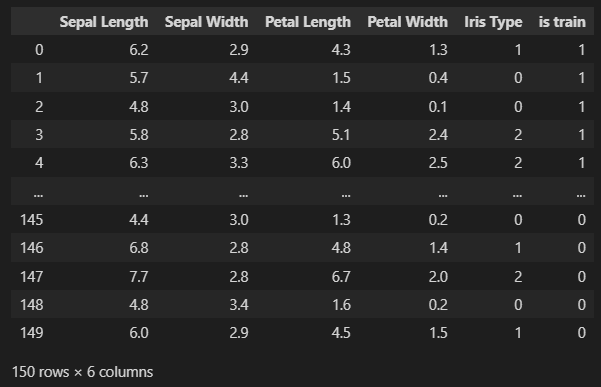
\includegraphics[width=0.7\linewidth]{../img/8}
	\caption{دیتاست}
	\label{fig:8}
\end{figure}
\subsection{تحلیل بصری داده}
در این بخش با در اختیار داشتن دیتاست، به رسم نمودار هایی از دیتاست و مشاهده داده های موجود در آن می پردازیم.
در بخش اول، دو ویژگی $Petal Length$ و $Petal Width$ از دیتاست را انتخاب کرده و توزیع آنها را نمایش می دهیم. این کار با استفاده از دستور jointplot از کتابخانه ی seaborn انجام می شود.
\begin{minted}{python}
import seaborn as sns
sns.jointplot(x=Dataset["Petal Length"], y=Dataset["Petal Width"],

kind="scatter", hue=Dataset["Iris Type"],palette="coolwarm")
\end{minted}
% TODO: \usepackage{graphicx} required
\begin{figure}[H]
	\centering
	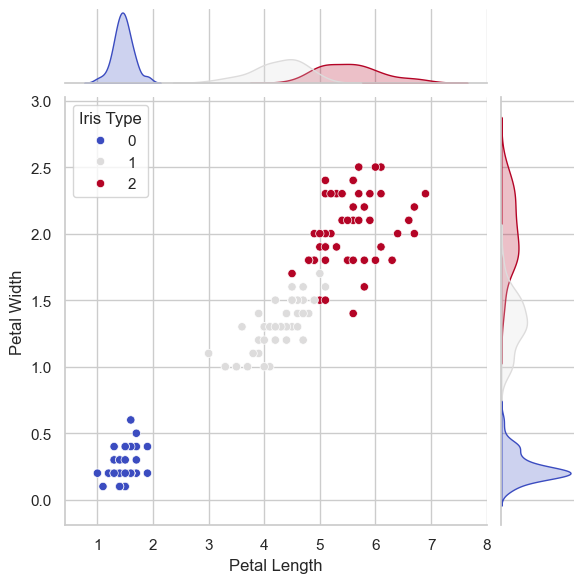
\includegraphics[width=1\linewidth]{../img/9}
	\caption{توزیع داده های $Petal Length$ و $Petal Width$ }
	\label{fig:9}
\end{figure}
در ادامه برای نمایش سه ویژگی از این دیتاست در یک نمودار سه بعدی به تفکیک نوع زنبق ها، از کتابخانه ی plotly استفاده می کنیم. در این روش، مقادیر دیتافریم در سه متغیر x و y و z تعریف شده و رنگ آن بر اساس نوع زنبق تعیین می شود.
پس از تعیین نمودار و برای بهبود آن، مارکر های قرار داده شده را تنظیم می کنیم و رنگ حاشیه آنها و ضخامت را تعیین می کنیم.
\begin{minted}{python}
import plotly.express as px

# Create the 3D scatter plot
fig = px.scatter_3d(Dataset,
x="Petal Length",
y="Petal Width",
z="Sepal Width",
color="Iris Type",  # Different colors for each species
color_discrete_sequence=px.colors.sequential.Magma, 
title="3D Scatter Plot of Iris Dataset")

# Customize markers
fig.update_traces(marker=dict(size=5,  # Marker size
opacity=0.8,  # Transparency
line=dict(width=10, color='black')),  # Black border around each point
selector=dict(mode='markers'))

# Add interactive layout settings
fig.update_layout(margin=dict(l=0, r=0, b=0, t=40),  # Remove margins
scene=dict(aspectmode='cube'))  # Equal scaling on all axes

# Show plot
fig.show()
\end{minted}
% TODO: \usepackage{graphicx} required
\begin{figure}[H]
	\centering
	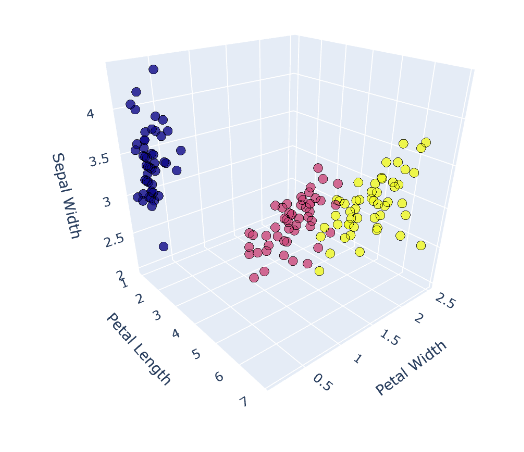
\includegraphics[width=0.7\linewidth]{../img/10}
	\caption{توزیع داده های سه وِیژگی سیستم}
	\label{fig:10}
\end{figure}
% TODO: \usepackage{graphicx} required
\begin{figure}[H]
	\centering
	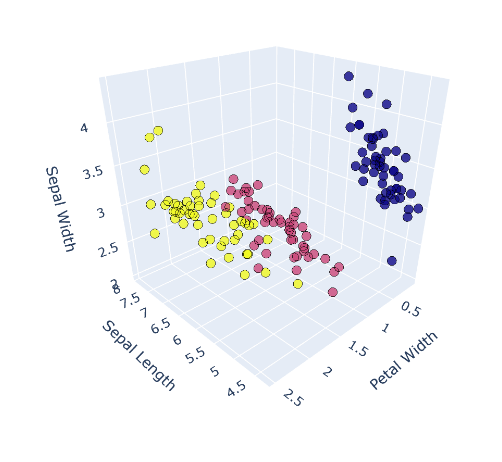
\includegraphics[width=0.7\linewidth]{../img/11}
	\caption{توزیع داده ها با سه ویژگی دیگر}
	\label{fig:11}
\end{figure}

در بخش بعد، برای بررسی شباهت فیچر های دیتاست با یکدیگر، ابتدا مقدار correlation آنها را به دست آورده و سپس نقشه حرارتی آن را رسم می کنیم.
\begin{minted}{python}
sns.heatmap(Dataset.corr(),annot=True )
plt.title("Correlation Heatmap")
\end{minted}
% TODO: \usepackage{graphicx} required
\begin{figure}[H]
	\centering
	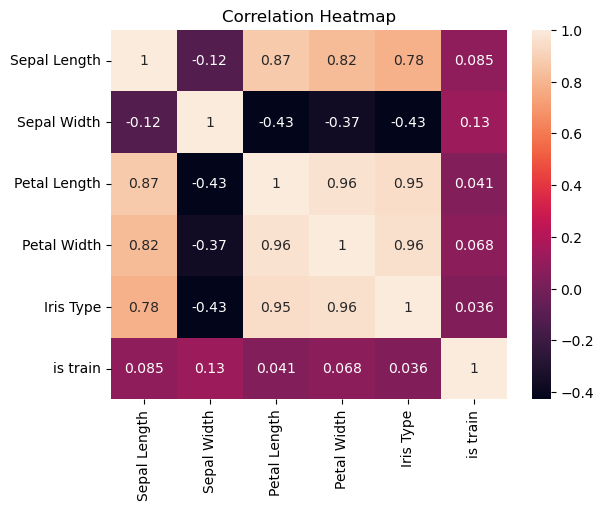
\includegraphics[width=0.7\linewidth]{../img/12}
	\caption{نمودار حرارتی correlation}
	\label{fig:12}
\end{figure}
در بخش بعد، به نمایش توزیع داده های هر فیچر به تفکیک داده های آموزش و تست می پردازیم. برای به دست آوردن این نمودارها، از دستور pairplot استفاده می شود. با اجرای این دستور برای دیتاست، توزیع دو به دوی تمامی فیچر ها نمایش داده می شود که بر روی قطر اصلی، توزیع هر ویژگی قابل مشاهده است.
\begin{minted}{python}
sns.pairplot(Dataset,hue='is train',palette='coolwarm')
\end{minted}
% TODO: \usepackage{graphicx} required
\begin{figure}[H]
	\centering
	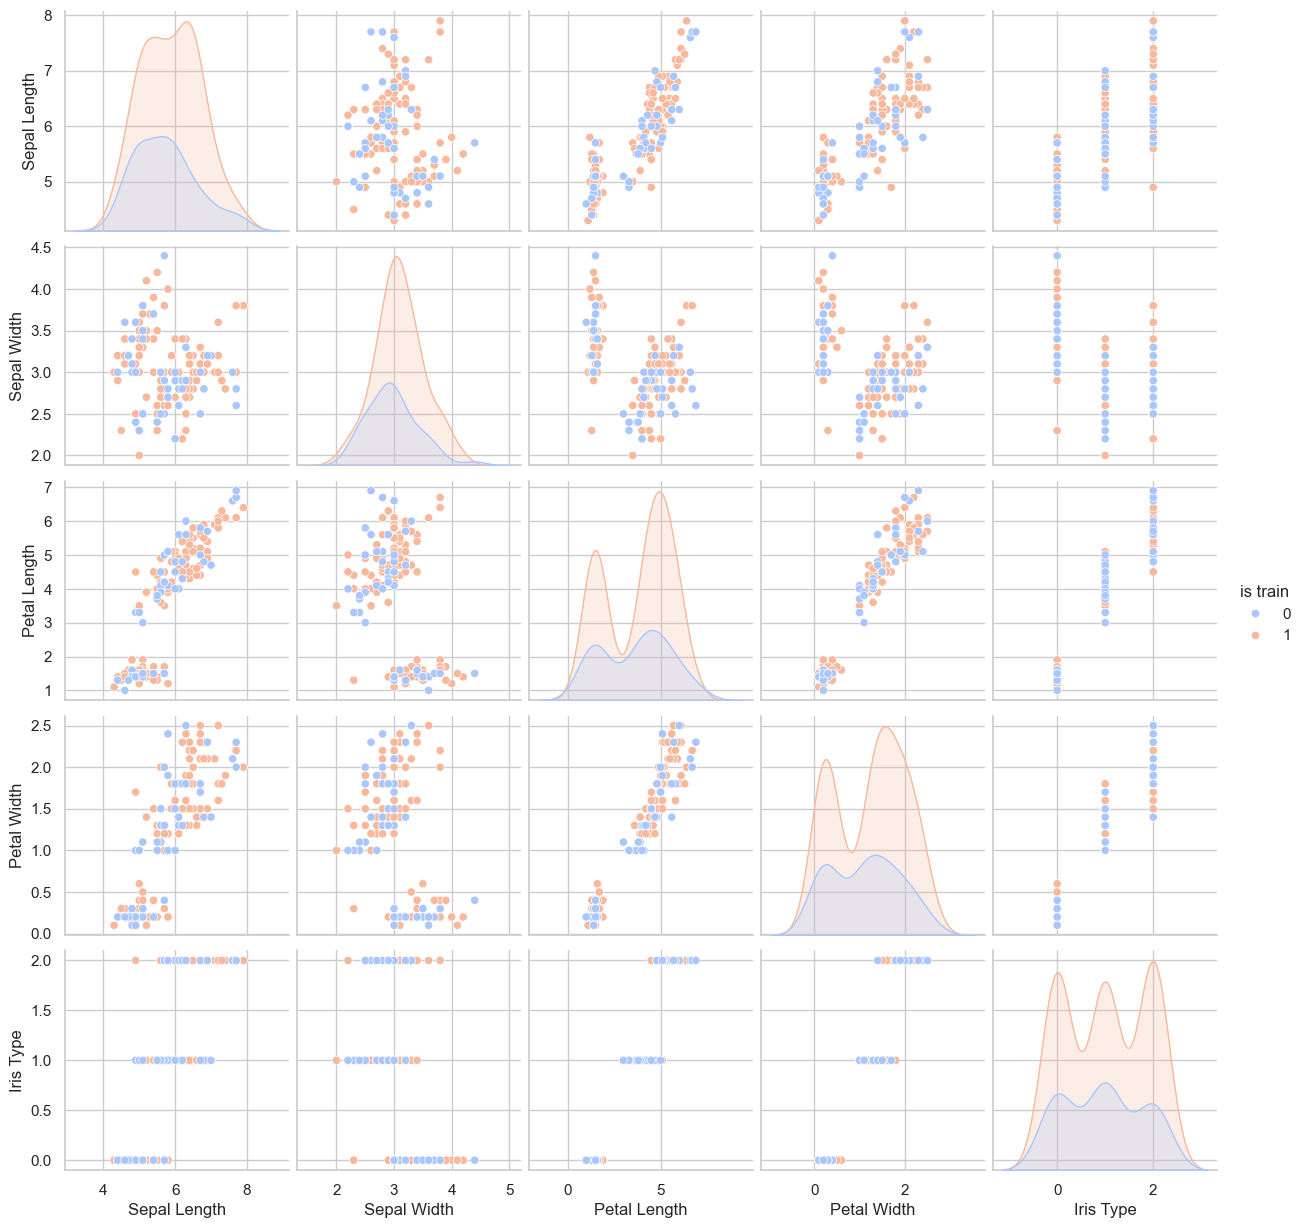
\includegraphics[width=1\linewidth]{../img/13}
	\caption{$Pair Plot$}
	\label{fig:13}
\end{figure}
\subsection{گسسته سازی}
در این بخش، ویژگی $petal length$ را گسسته می کنیم. برای این کار، تعداد دسته های مورد نیاز و عنوان آنها را تعریف کرده و سپس با استفاده از دستور cut از کتابخانه ی pandas، مقادی را در بازه های مورد نظر دسته بندی می کنیم.
\begin{minted}{python}
bins = 3  # Number of categories
labels = ["Short", "Medium", "Tall"]  # Custom labels
Dataset["Discrit Petal Lemgth"]=pd.cut(Dataset["Petal Length"], bins=bins, labels=labels)
\end{minted}
در این صورت، دیتاست نهایی به صورت زیر به دست می آید.
% TODO: \usepackage{graphicx} required
\begin{figure}[H]
	\centering
	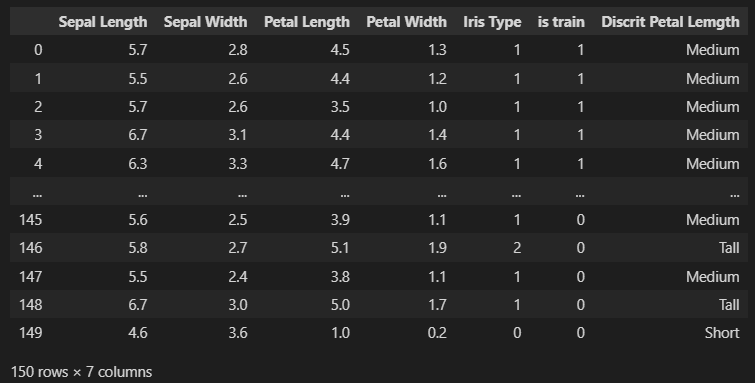
\includegraphics[width=0.7\linewidth]{../img/14}
	\caption{دیتاست پس از گسسته سازی}
	\label{fig:14}
\end{figure}
\subsection{تحلیل آماری}
در گام آخر، دیتاست را با استفاده از متد describe، توصیف کرده و پارامتر های آماری آن را محاسبه می کنیم. در اینجا تنها شرط آن را قرار می دهیم که تنها داده هایی با $Iris Type$ برابر با 0 که معادل Setosa است آورده شود.
\begin{minted}{python}
Dataset[Dataset["Iris Type"] ==0].describe()
\end{minted}
% TODO: \usepackage{graphicx} required
\begin{figure}[H]
	\centering
	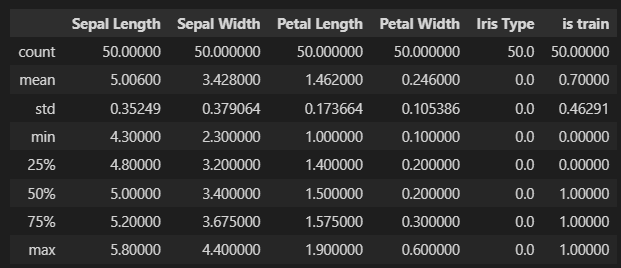
\includegraphics[width=0.7\linewidth]{../img/15}
	\caption{تحلیل آماری داده های ستوسا}
	\label{fig:15}
\end{figure}







	



 
 
 
 